\begin{table}[H]
\centering
\begin{tabular}{@{}lll@{}}
\toprule
\textbf{Aspect} & \textbf{Axion} & \textbf{Électron} \\ \midrule
Masse & \(10^{-5}\) eV & 511 keV \\
Longueur d'onde & \(0,124\) m & \(2,4\times10^{-12}\) m \\
Comportement & Onde & Particule \\
Interaction & Très faible & Électromagnétique \\
Rôle dans ART-12D & Mode du champ akashique & Récepteur neuronal \\ \bottomrule
\end{tabular}
\end{table}

\subsection{Quelles particules traversent votre corps ?}
La matière noire a une densité locale d'environ 0,3 GeV/cm$^3$ (Read, 2014). La densité numérique dépend toutefois de la masse, $n = \rho/m$, et le flux est $\Phi = n v$. Pour un mode de $10^{-5}$ eV et $v = 300$ km/s, on obtient :
\begin{equation}
n = \frac{0,3 \times 10^{15}\ \text{eV/m}^3}{10^{-5}\ \text{eV}} = 3,0\times10^{19}\ \text{m}^{-3},
\qquad
\Phi = n v = 9,0\times10^{24}\ \text{m}^{-2}\text{s}^{-1}.
\end{equation}
Pour un corps humain d'une surface de 0,7 m$^2$ :
\begin{equation}
\Phi_{\text{body}} = 9,0\times10^{24} \times 0,7 \approx 6\times10^{24} \text{ particles/s}.
\end{equation}
Environ $6\times10^{24}$ particules par seconde. (La version 30 affirmait $n = 3000$ m$^{-3}$ et $6\times10^8$ s$^{-1}$ ; ces valeurs correspondent à un WIMP d'environ 100 GeV, non à un mode de $10^{-5}$ eV.)

\begin{figure}[H]
\centering
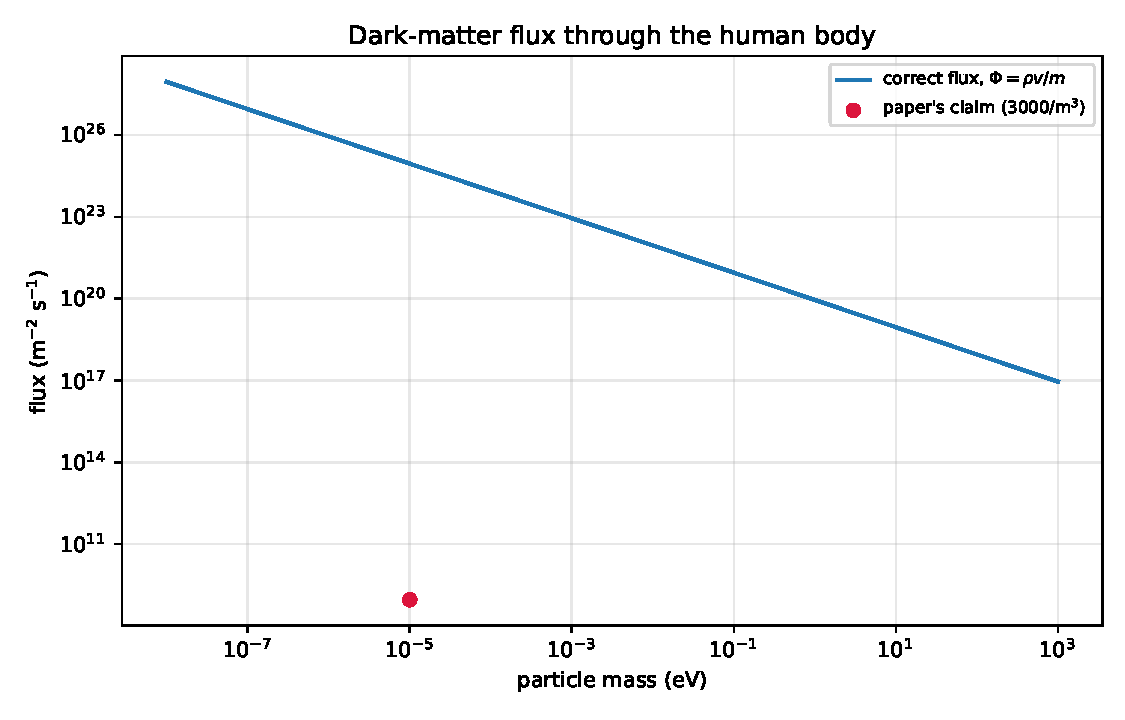
\includegraphics[width=0.82\textwidth]{figures/fig07_flux.pdf}
\caption{Le flux de matière noire à travers le corps humain en fonction de la masse de la particule. Le point rouge marque l'affirmation de la version 30 ; la courbe est la valeur correcte pour $\rho = 0,3$ GeV/cm$^3$ et $v = 300$ km/s. À $10^{-5}$ eV, la différence est de 16 ordres de grandeur.}
\label{fig:flux}
\end{figure}

\subsection{Que deviennent ces particules ?}
La plupart vous traversent sans interagir. Quelques-unes interagissent avec les noyaux atomiques : indépendamment du spin ($\sim 5$ collisions/an), dépendamment du spin ($\sim 30$ collisions/an). L'effet sur le corps : radiation naturelle ($\sim 2,4$ mSv/an) ; matière noire ($\sim 10^{-15}$ mSv/an).

\subsection{Comment détecte-t-on ces particules ?}
Détecteurs directs : LUX-ZEPLIN (10 tonnes de xénon) --- sensibilité : $10^{-48}$ cm$^2$. Détecteurs indirects : Fermi-LAT (recherche de rayons gamma d'annihilation), ADMX (recherche d'axions). Section efficace : $\sigma \sim 10^{-47}$ cm$^2$. Probabilité d'interaction : $P \sim 10^{-22}$.

\subsection{La matière noire comme onde, non comme particules}
Si la matière noire est un champ scalaire, elle n'est pas composée de particules individuelles. C'est une onde qui remplit l'univers. Formalisation : $A(x,t) = \sum_n A_n \cos(\omega_n t + \varphi_n)$.

\subsection{L'analogie de l'arbre et du photon}
Imaginez un arbre sur une plage. Le soleil brille. Les photons quittent le soleil avec l'énergie $E = h\nu$. Ils atteignent l'arbre. Ils sont absorbés par chaque feuille avec la même énergie $h\nu$. Comment un seul photon peut-il atteindre toutes les feuilles avec la même énergie ? S'il était une particule, il perdrait de l'énergie à chaque collision. Or il ne le fait pas. La réponse est simple : parce que le photon est une onde, non une particule. Une onde ne se « consume » pas en traversant la matière. Elle s'étend sur tout l'espace. Chaque feuille « voit » l'onde entière. L'état du photon : $|\psi_{\text{photon}}\rangle = \int d^3k \, c(k) |k\rangle$.

\subsection{La dualité onde--particule comme mécanisme de traversée}
Si la matière ne peut traverser entre les univers (car cela exigerait une énergie infinie) et que les univers sont reliés par la matière noire, comment communiquent-ils ? La réponse d'ART-12D : par la dualité onde--particule. Étape 1 : la matière devient onde. $|\text{particle}\rangle_A \to |\text{wave}\rangle_A$. Étape 2 : l'onde traverse. $|\text{wave}\rangle_A \to |\text{wave}\rangle_B$. Étape 3 : l'onde devient particule. $|\text{wave}\rangle_B \to |\text{particle}\rangle_B$. Étape 4 : l'information est transduite. $I_A \to I_B$.

\subsection{Le spectre émotionnel humain}
Les sentiments humains se répartissent en deux grandes catégories : positifs et négatifs. Chaque sentiment a une fréquence caractéristique et un effet spécifique sur la conscience. Formalisation : $S_{\text{total}} = \sum_{i=1}^{48} S_i^{\text{positive}} + \sum_{j=1}^{46} S_j^{\text{negative}}$. Voici un extrait du tableau étendu (la version complète figure en annexe B) :
\begin{table}[H]
\centering
\begin{tabular}{@{}lll@{}}
\toprule
\textbf{Sentiment} & \textbf{Fréquence dominante (Hz)} & \textbf{Effet} \\ \midrule
Joie & 400-600 & Expansion, dynamisme \\
Paix & 200-350 & Calme réflexif \\
Amour & 200-400 & Émotion profonde \\
Gratitude & 300-500 & Contentement \\
Peur & 500-800 & Active l'amygdale \\
Colère & 600-800 & Rage \\
Tristesse & 400-600 & Mélancolie \\
Envie & 600-800 & Jalousie \\ \bottomrule
\end{tabular}
\end{table}
Les fréquences musicales thérapeutiques (432 Hz, 528 Hz, 639 Hz, 741 Hz, 852 Hz, 963 Hz) ont été corrélées aux fréquences du champ akashique. Les sept sens humains comprennent cinq sens physiques (vue, ouïe, odorat, goût, toucher) et deux sens psychiques (imagination, empathie).

\subsection{Le cœur comme modulateur de la réception}
Le cœur possède son propre système électrique (le nœud sinusal) qui génère des impulsions indépendamment du cerveau. Il fonctionne comme un modulateur de la réception, non comme un récepteur indépendant. Le cerveau est le récepteur principal, le cœur ajuste la cohérence. Formalisation : $C_{\text{coherent}} = C_0 \times (1 + \beta \times HRV)$. Les chiffres scientifiques exacts : le cerveau consomme environ $20$ W de puissance métabolique, le cœur fournit environ $1-1,3$ W de puissance mécanique, mais produit des champs électriques et magnétiques d'amplitude bien plus grande.

\subsection{Le mot qui peut remplacer n'importe quel médicament}
L'hypothèse : $L_{\text{word-matter}} = g_{CM} A_{\text{meaning}} \psi \psi$. Ce que le mot peut faire : $Effect_{\text{total}} = Effect_{\text{medicine}} + Effect_{\text{word}} + \text{Interaction}$. Ce que le mot ne peut pas faire : il ne peut pas remplacer les antibiotiques contre les infections bactériennes, il ne peut pas remplacer l'insuline dans le diabète de type 1, il ne peut pas remplacer la chirurgie en cas d'appendicite, il ne peut pas remplacer la chimiothérapie contre le cancer. Prédiction 67 : l'effet du mot.

\newpage
